\documentclass{beamer}
 
\usepackage[utf8]{inputenc}

\usepackage[newfloat]{minted}

\usepackage{pgf}
\usepackage{tikz}
\usepackage{upquote}
\usetikzlibrary{arrows,automata}

\newenvironment{code}{\captionsetup{type=listing}}{}
\SetupFloatingEnvironment{listing}{name=Listing}

\title{An Introduction To Dependent Types}
\author{Donovan Crichton}
\date{February 2018}

\begin{document}
 
\frame{\titlepage}

\begin{frame}[fragile]
  \frametitle{A Brief Definition.}

  \begin{block}{What are dependent types?}
  \begin{itemize}
    \item A dependent type is a type whose complete definition depends on
  some value. 

    \item This is very different to an ordinary paramterised ADT, where the
  definition depends on the \alert{type} of the paramter(s) only.
  \end{itemize}
  \end{block}
  \begin{block}{Ordinary ADT}
  \begin{minipage}{0.5\textwidth}
  \begin{minted}{haskell}
  data MyType a = MyStr String a | MyInt Int a
  \end{minted}
  \end{minipage}
  \end{block}
\end{frame}

\begin{frame}[fragile]
\frametitle{Recursive ADTs}
  \begin{minipage}{1\textwidth}
  \begin{minted}{haskell}
  data Expr a
    = I Int 
    | B Bool 
    | Add (Expr Int) (Expr Int) 
    | And (Expr Bool) (Expr Bool)

  --eval Int
  f :: Expr a -> Maybe Int
  f (I x)     = Just x
  f (Add x y) = pure (+) <*> (f x) <*> (f y)
  f _         = Nothing
 
  --eval Bool
  g :: Expr a -> Maybe Bool
  g (B x)     = Just x
  g (And x y) = pure (&&) <*> (g x) <*> (g y)
  g _         = Nothing
  \end{minted}
  \end{minipage}
\end{frame}

\begin{frame}[fragile]
\frametitle{Type Class to the Rescue!}
\begin{minipage}{1\textwidth}
\begin{minted}{haskell}
  data Expr a
    = I Int 
    | B Bool 
    | Add (Expr Int) (Expr Int) 
    | And (Expr Bool) (Expr Bool)

  class Eval a where
    eval :: Expr a -> a

  instance Eval Int where
    eval (I x)     = x
    eval (Add x y) = (eval x) + (eval y)

  instance Eval Bool where
    eval (B x)     = x
    eval (And x y) = (eval x) && (eval y)
\end{minted}
\end{minipage}
\end{frame}

\begin{frame}[fragile]
\frametitle{Recursive ADTs - Problems}
\begin{itemize}
\item We'd like a way to apply a single function (eval) to our class of type
  constructors (Expr).
\item Type classes work for the previous example, but things start to go pear
  shaped when we want to constrain our type constructors with type classes.
\item More complicated expressions require multiple type parameters that are
only used by a few type constructors.
\item This example requires a deprecated extension, is generally
considered poor practice, and more constraints = more type parameters! \\
\end{itemize}
\begin{minipage}{1\textwidth}
  \begin{minted}{haskell}
  data Num a => Expr a
    = N a
    | B Bool
    | Add (Expr a) (Expr a)
    | And (Expr Bool) (Expr Bool)
  \end{minted}
\end{minipage}
\end{frame}

\begin{frame}[fragile]
\frametitle{GADTs}
  \begin{itemize}
    \item Generalised Algebraic Data Types (or Dependent Data Types) are a
      generalisation of ADTs, hence the name.
    \item The development of GADTs was strongly motivated by this restriction
      on type class constraints, particularly on their decomposition.
    \item Particularly useful when you want to generalise a function across a 
      class or family of data.
  \end{itemize}
  \begin{minipage}{1\textwidth}
  \end{minipage}
\end{frame}

\begin{frame}[fragile]
\frametitle{GADTs - An Example}
  \begin{minipage}{1\textwidth}
    \begin{minted}{haskell}
      {-# LANGUAGE GADTs #-}
      data Expr a where
        Lift :: (Show a) => a -> Expr a
        Add  :: Num a => Expr a -> Expr a -> Expr a
        And  :: Expr Bool -> Expr Bool -> Expr Bool

      -- now this works!
      eval :: Expr a -> a
      eval (Lift x)  = x
      eval (Add x y) = (eval x) + (eval y)
      eval (And x y) = (eval x) && (eval y)
    \end{minted}
  \end{minipage}
\end{frame}

\begin{frame}[fragile]
\frametitle{GADTs - Other Information}
  \begin{itemize}
    \item The a's inside the constructor definition are \textit{only} given
      their explicit types through pattern matching! 
      This can cause problems for the unwary.
    \item The type parameter of a GADT is \textit{dependent} on the type
      constructor used to construct the data type. Thus GADTs are a simple form
      of a dependent type.
    \item GADTs can be used to treat a group of different, but related things
      in a similar way (but that may be different for each specific thing).
  \end{itemize}
\end{frame}

\begin{frame}[fragile]
\frametitle{GADTS - Validated State Transitions}
GADTs can also be used to have the type-checker validate transitions in a 
finite state machine. Lets consider an automatic door: \\
\\
\begin{minipage}{1\textwidth}
\begin{center}
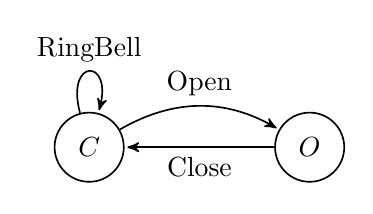
\begin{tikzpicture}[->,>=stealth',shorten >=1pt,auto,node distance=2.8cm,
                    semithick]

  \node[state] (DoorClosed)                    {$C$} ;
  \node[state] (DoorOpen) [right of=DoorClosed]  {$O$};

  \path (DoorClosed) edge [bend left, above]  node {Open} (DoorOpen);
  \path (DoorClosed) edge [loop above] node {RingBell} (DoorClosed);
  \path (DoorOpen)   edge [right, below] node {Close} (DoorClosed);
\end{tikzpicture}
\end{center}
\end{minipage}
\end{frame}

\begin{frame}[fragile, shrink=10]
\frametitle{Validated FSMs - An Example}
\begin{minted}{haskell}
{-# LANGUAGE GADTs #-}
{-# LANGUAGE DataKinds #-}
{-# LANGUAGE KindSignatures #-}

data DoorState = DoorOpen | DoorClosed

data DoorCmd :: DoorState -> DoorState -> * -> * where
  Open     :: DoorCmd DoorClosed DoorOpen   ()  
  Close    :: DoorCmd DoorOpen   DoorClosed ()
  RingBell :: DoorCmd DoorClosed DoorClosed ()
  Pure     :: a -> DoorCmd state state a
  Bind     :: DoorCmd state1 state2 a -> 
              (a -> DoorCmd state2 state3 b) ->
              DoorCmd state1 state3 b

-- this will throw a type error!
doorProg :: DoorCmd DoorClosed DoorClosed ()
doorProg = Open `Bind` \x ->  
           RingBell
\end{minted}
\end{frame}

\begin{frame}[fragile, shrink=10]
\frametitle{Validated FSMs - A (Correct) Example}
\begin{minted}{haskell}
{-# LANGUAGE GADTs #-}
{-# LANGUAGE DataKinds #-}
{-# LANGUAGE KindSignatures #-}

data DoorState = DoorOpen | DoorClosed

data DoorCmd :: DoorState -> DoorState -> * -> * where
  Open     :: DoorCmd DoorClosed DoorOpen   ()  
  Close    :: DoorCmd DoorOpen   DoorClosed ()
  RingBell :: DoorCmd DoorClosed DoorClosed ()
  Pure     :: a -> DoorCmd state state a
  Bind     :: DoorCmd state1 state2 a -> 
              (a -> DoorCmd state2 state3 b) ->
              DoorCmd state1 state3 b

-- this works!
doorProg :: DoorCmd DoorClosed DoorClosed ()
doorProg = RingBell `Bind` \x ->  
           Open `Bind` \y -> 
           Close
\end{minted}
\end{frame}

\begin{frame}[fragile]
\frametitle{Closed Type Families}
  \begin{itemize}
    \item A stronger form of dependent type than a GADT. Closed Type Families
      (Type-Level Functions in Idris) allow computations to be expressed at 
      the type level!
    \item This in practice allows you to write more expressive types, and
      exclude a greater number of invalid programs at compile time.
    \item Haskell does not fully support dependent types yet, but can get
      fairly close with a fair amount of work.
    \item Key Haskell extensions are: DataKinds, KindSignatures, GADTs,
          TypeFamilies and TypeOperators, along with knowledge of the
          singletons library and Template Haskell.
  \end{itemize} 
\end{frame}

\begin{frame}[fragile]
\frametitle{Type-Level Functions}
Typel-level functions allow a function from a value input, to a type output.
These then get paired with an ordinary (value-level) function which returns a
type of the type-level function: \\ \\
\begin{minipage}{1\textwidth}
\begin{minted}{haskell}
  IntOrString : Bool -> Type
  IntOrString True = Int
  IntOrString False = String

  intOrString : (x : Bool) -> IntOrString x
  intOrString True  = 6
  intOrString False = "Six"
\end{minted}
\end{minipage}
\end{frame}

\begin{frame}[fragile]
\frametitle{First Class Types}
\begin{itemize}
\item In order for the previous slide to work, functions have to be able to
return types.
\item This suggests that variables must also accept types.
\item This further suggests that types must be a first class construct!
\item If types are a first class construct then we can use types anywhere we
can use a function, which is anywhere we can use a value.
\item This also means we can use functions or values where we can use types!
\end{itemize}
\end{frame}

\begin{frame}[fragile]
\frametitle{Vectors - The Obligatory Example}
\begin{minipage}{1\textwidth}
Through both dependent data-types (GADTs) and type-level \\
functions (closed type families) we can express stronger type constraints: \\ 
  \begin{minted}{haskell}
  infixr 5 ::: 

  data Vec : Nat -> Type -> Type where
    VNil : Vec 0 a 
    (:::) : (x : a) -> (xs : Vec n a) -> Vec (n + 1) a

  x : Vec 3 Char
  x = 'a' ::: 'b' ::: 'c' ::: VNil

  -- this wont typecheck!
  y : Vec 4 Char
  y = 'a' ::: 'b' ::: 'c' ::: VNil
  \end{minted}
\end{minipage}
\end{frame}

\begin{frame}[fragile, shrink=5]
\frametitle{Vectors in Haskell}
\begin{minted}{haskell}
{-# LANGUAGE GADTs #-}
{-# LANGUAGE DataKinds #-}
{-# LANGUAGE KindSignatures #-}

infixr 5 ::: 

data Nat = Z | S Nat 

data Vec :: Nat -> * -> * where
  Nil :: Vec Z a 
  (:::) :: a -> Vec n a -> Vec (S n) a

x :: Vec (S (S (S Z))) Char
x = 'a' ::: 'b' ::: 'c' ::: Nil 

--this will not typecheck
y :: Vec (S (S (S (S Z)))) Char
y = 'a' ::: 'b' ::: 'c' ::: Nil 
\end{minted}
\end{frame}

\begin{frame}[fragile]
\frametitle{Constraints as Types}
\begin{itemize}
\item Program constraints can be lifted to the type level, through the use of
  functions as types.
\item This causes the type checker to act as a kind of proof checker! It is no
  coincidence that the early dependently typed languages were focused on
  theorem proving!
\item Complexity can be added to the program types as required, in a kind of
  pay-as-you-go approach.
\item You're paying in verbosity! Type-level functions are required to be total
  in Idris, which means they must be defined for \textit{every} possible case.
\item You're also paying in design complexity, the more elbarate the type
  computation, the more difficult it is to reason about the types involved.
\item Still worth it though!
\end{itemize}


\end{frame}

\end{document}

